\documentclass[11pt,a4paper]{article}

\usepackage[margin=1in]{geometry}
\usepackage{graphicx}
\usepackage{booktabs}
\usepackage{amsmath}
\usepackage{amssymb}
\usepackage{natbib}
\usepackage{hyperref}
\usepackage{caption}
\usepackage{subcaption}
\usepackage{enumitem}
\usepackage{tikz}
\usetikzlibrary{arrows.meta, positioning, shapes.geometric, calc}
\usepackage{algorithm}
\usepackage{algpseudocode}
\usepackage{xcolor}

\hypersetup{
  colorlinks=true,
  linkcolor=blue!70!black,
  citecolor=blue!70!black,
  urlcolor=blue!70!black
}

\title{\textbf{Down Round as Emergent Strategy:\\Multi-Agent RL Evidence from Venture Capital Auctions}}

\author{
  Xinglin Lai\\
  Department of Finance, Lingnan University\\
  \texttt{xinglinlai@ln.hk} \quad \texttt{xinglinzephyrlai@gmail.com}
}

\date{May 2026}

\begin{document}

\maketitle

\begin{abstract}
Down rounds---financing rounds where post-money valuation falls below the previous round---are prevalent in venture capital, occurring in nearly half of consecutive funding sequences. We ask: are they purely statistical artifacts of noisy valuations, or do rational agents strategically devalue? Using a data-calibrated multi-bidder Vickrey auction environment with MAPPO agents under Centralized Training Decentralized Execution (CTDE), we demonstrate that Down Round rate rises from 49\% (random baseline, matching empirical data's 49.35\%) to 82\% after reinforcement learning training---a 33\% \emph{strategic component} that emerges as rational optimal behavior. However, RL-trained agents produce mild Down Rounds (-29\% magnitude), far less severe than real data (-62\%), revealing a ``magnitude paradox'' likely explained by behavioral biases. We propose an RL+LLM+Data merge framework where Direct Preference Optimization (DPO)-trained LLMs decode RL strategies and quantify bias contributions, bridging reinforcement learning emergence with LLM post-training interpretability for agentic AI in business research.
\end{abstract}

\section{Introduction}

In venture capital financing, a \emph{down round} occurs when a company raises capital at a post-money valuation lower than its previous round. This phenomenon is not rare: among consecutive funding sequences in our dataset of 49,996 rounds, down rounds constitute 49.35\% of events. Yet the fundamental question---\emph{why} do down rounds occur?---remains poorly understood despite extensive literature proposing five distinct mechanisms: statistical effects, intertemporal arbitrage, information cascades, market structure, and behavioral biases \citep{milgrom1982,gompers1998,kahneman1979}.

Traditional econometric approaches face three fundamental obstacles: (1) \textbf{data sparsity}---only $\sim$1\% of Crunchbase rounds contain valuation data; (2) \textbf{identification difficulty}---separating statistical, strategic, and behavioral contributions requires counterfactuals unavailable in observational data; (3) \textbf{conflicting theories}---different mechanisms predict similar outcomes, making causal attribution impossible.

Our approach addresses these limitations through a \emph{computational randomized controlled trial}: we construct a multi-agent reinforcement learning (RL) environment that mirrors the essential economics of VC auctions, train agents to learn optimal bidding strategies, and analyze what behaviors \emph{emerge}. If down rounds are rational optimal strategies, they should emerge spontaneously in sufficiently trained RL agents---analogous to how chain-of-thought reasoning and in-context learning emerge in large language models \citep{brown2020,wei2022}.

This paper presents Phase A of an RL+LLM+Data merge framework, demonstrating three core findings:
\begin{enumerate}[nosep]
  \item \textbf{Emergence}: Down rounds emerge as rational strategy, adding a 33\% strategic component beyond the 49\% statistical baseline.
  \item \textbf{Magnitude paradox}: RL agents produce frequent but mild DRs (-29\%), while real data shows severe DRs (-62\%), suggesting behavioral amplification.
  \item \textbf{Phase transition}: DR emergence follows a phase-transition pattern across noise and prior-price deviation dimensions.
\end{enumerate}

Phase B (planned) connects RL emergence to LLM post-training via DPO \citep{rafailov2023}, enabling LLMs to ``decode'' RL black-box strategies and quantify behavioral bias contributions---a novel agentic AI application for business research.

\section{Related Work}

\subsection{Auction Theory and Down Rounds}

The Vickrey (second-price) auction \citep{vickrey1961} provides the theoretical foundation for our environment. In common-value auctions, the winner's curse \citep{thaler1988} creates systematic overbidding, and the linkage principle \citep{milgrom1982} shows how public information reduces this effect. Our model extends this to a \emph{multi-period} setting where inter-round value shifts and ownership dilution create cross-period strategic incentives \citep{gompers1998}.

\subsection{RL Emergence and Multi-Agent Learning}

Recent work on LLM scaling reveals that qualitatively new capabilities emerge beyond parameter thresholds \citep{wei2022}. We apply this insight to RL: if down rounds are optimal, they should \emph{emerge} during training rather than require explicit programming. MAPPO with CTDE architecture \citep{yu2021}, building on MADDPG \citep{lowe2017} and PPO \citep{schulman2017}, enables information asymmetry modeling where actors use private signals and critics observe global states.

\subsection{LLM Post-Training and Interpretability}

DPO \citep{rafailov2023} directly optimizes language models from preference data without a separate reward model, contrasting with RLHF \citep{outrihed2023,christiano2017}. Our Phase B applies DPO to train LLMs as ``decision interpreters''---generating reasoning chains that explain RL agent actions and distinguish rational from biased decision logic. This bridges RL interpretability with agentic AI \citep{wang2023}.

\section{Model Design}

\subsection{Auction Environment}

We model VC financing as a two-period Vickrey auction with inter-round value shifts:

\begin{itemize}[nosep]
  \item \textbf{Agents}: $N=3$ bidders compete in each round (matching typical VC round investor count)
  \item \textbf{Valuation}: Stochastic $V$ per episode from log-normal ($\text{median}=100$, $\sigma_{\log}=1.19$, calibrated from data), with inter-round shift: $V_1 = V \cdot e^{\mathcal{N}(0, \sigma_{\text{shift}})}$ where $\sigma_{\text{shift}}=1.0$
  \item \textbf{Signals}: Each bidder receives private signal $\theta_i \sim \mathcal{N}(V_t, \sigma^2)$ with $\sigma/V \approx 20\%$ and adaptive noise scaling
  \item \textbf{Ownership}: Winner acquires fraction $\alpha = 0.17$ (median funding/valuation ratio from data)
\end{itemize}

The stochastic valuation mechanism is the key calibration innovation: drawing $V$ from a log-normal distribution ($\sigma_{\log}=1.19$, calibrated from Openbook data) and applying inter-round shifts ($\sigma_{\text{shift}}=1.0$) produces a random baseline DR rate of $\sim$48\% (close to data's 49.35\%), reflecting real-world valuation volatility across episodes and between financing rounds.

\subsection{MAPPO CTDE Architecture}

We adopt Centralized Training Decentralized Execution (CTDE) to model the natural information asymmetry in VC markets:

\textbf{Decentralized Actor} (6-dim input): $[\theta_i, t, P_0, w_{i}^{prev}, \mu_{belief}, \sigma_{belief}]$ $\rightarrow$ bid $b_i$
\begin{itemize}[nosep]
  \item Two-layer MLP: $\text{obs\_dim} \rightarrow 64 \rightarrow 64 \rightarrow 1$
  \item Gaussian policy: $b_i \sim \mathcal{N}(\mu(\theta_i), \sigma^2)$
  \item Only uses \emph{private} observation during execution
\end{itemize}

\textbf{Centralized Critic} (9-dim input for $N=3$): $[\theta_0, \theta_1, \theta_2, t, P_0, w^{prev}, o_0, o_1, o_2]$ $\rightarrow$ $V(s)$
\begin{itemize}[nosep]
  \item Deeper network: $9 \rightarrow 128 \rightarrow 128 \rightarrow 64 \rightarrow 1$
  \item Observes \emph{all} agent signals and ownership during training
  \item Enables more accurate value estimation despite execution-time information asymmetry
\end{itemize}

\subsection{Reward Function}

Rewards incorporate ownership dilution and cross-round optionality:
\begin{align}
R_0^{winner} &= \alpha \cdot V - P_0 + \gamma \cdot (1-\alpha) \cdot \alpha \cdot V \cdot \frac{0.5}{N} \\
R_1^{winner} &= \alpha' \cdot V_1 - P_1
\end{align}
where $\alpha' = (1 - o_{total}) \cdot \alpha$ accounts for dilution, and $V_1$ uses the shifted valuation. Round 0 rewards include a future option value term reflecting the strategic benefit of early ownership for subsequent rounds.

\subsection{Belief Update}

After Round 0, agents update beliefs about opponent signals via simplified Bayesian inference:
\begin{equation}
\mu_{post} = \frac{\mu_{prior}/\sigma_{prior}^2 + P_0/\sigma_{obs}^2}{1/\sigma_{prior}^2 + 1/\sigma_{obs}^2}
\end{equation}
where $\sigma_{obs} = 1.5\sigma$, treating the observed price as a noisy signal about the opponent's type.

\section{Results}

\subsection{Calibration to Empirical Data}

The stochastic valuation and v\_shift mechanism ($\sigma_{\log}=1.19$, $\sigma_{\text{shift}}=1.0$) produces a random baseline that closely matches key data statistics (Table~\ref{tab:calibration}). Untrained agents bidding proportionally to their signals yield DR statistics that approximate the empirical distribution without any strategic learning.

\begin{table}[t]
\centering
\caption{Random baseline vs. empirical data statistics. The stochastic V ($\sigma_{\log}=1.19$) plus v\_shift ($\sigma_{\text{shift}}=1.0$) produces a statistical baseline closely matching data.}
\label{tab:calibration}
\begin{tabular}{lcc}
\toprule
\textbf{Statistic} & \textbf{Data} & \textbf{Random Baseline} \\
\midrule
DR rate (consecutive) & 49.35\% & 48\% \\
DR magnitude (mean) & -62.24\% & close match \\
DR magnitude (median) & -68.11\% & close match \\
Ownership median & 0.17 & 0.17 \\
\bottomrule
\end{tabular}
\end{table}

\subsection{Strategic Emergence of Down Rounds}

After 10,000 episodes of MAPPO training with $N=3$ bidders, DR rate rises from 49\% to 82\%, demonstrating a \textbf{33\% strategic component} (Table~\ref{tab:results}). This emergence is consistent with Hypothesis H1: down rounds arise as rational optimal strategies when agents learn to exploit inter-round value shifts and ownership dynamics.

\begin{table}[t]
\centering
\caption{Key experimental results. RL training adds a 33\% strategic component to DR rate but reduces DR magnitude, creating the magnitude paradox.}
\label{tab:results}
\begin{tabular}{lccc}
\toprule
\textbf{Statistic} & \textbf{Random} & \textbf{RL-Trained} & \textbf{Strategic} \\
 & \textbf{Baseline} & & \textbf{Component} \\
\midrule
DR rate & 49\% & \textbf{82\%} & +33\% \\
DR magnitude (mean) & -40\% & \textbf{-29\%} & milder \\
DR magnitude (median) & -38\% & \textbf{-24\%} & milder \\
\bottomrule
\end{tabular}
\end{table}

\subsection{Equilibrium Policy Functions}

Figure~\ref{fig:policy} reveals the learned bidding strategies for three agents. In Round 0 (left panel), all three agents bid above the stake-value benchmark ($b = 0.17\theta$), reflecting competitive pressure among three bidders. In Round 1 (right panel), all agent strategies systematically fall below $P_0$ for most price levels, placing their bids in the down round region ($b_1 < P_0$). This confirms that down rounds are the \emph{equilibrium outcome} of rational bidding with multiple competing investors, not merely statistical noise.

\begin{figure}[t]
\centering
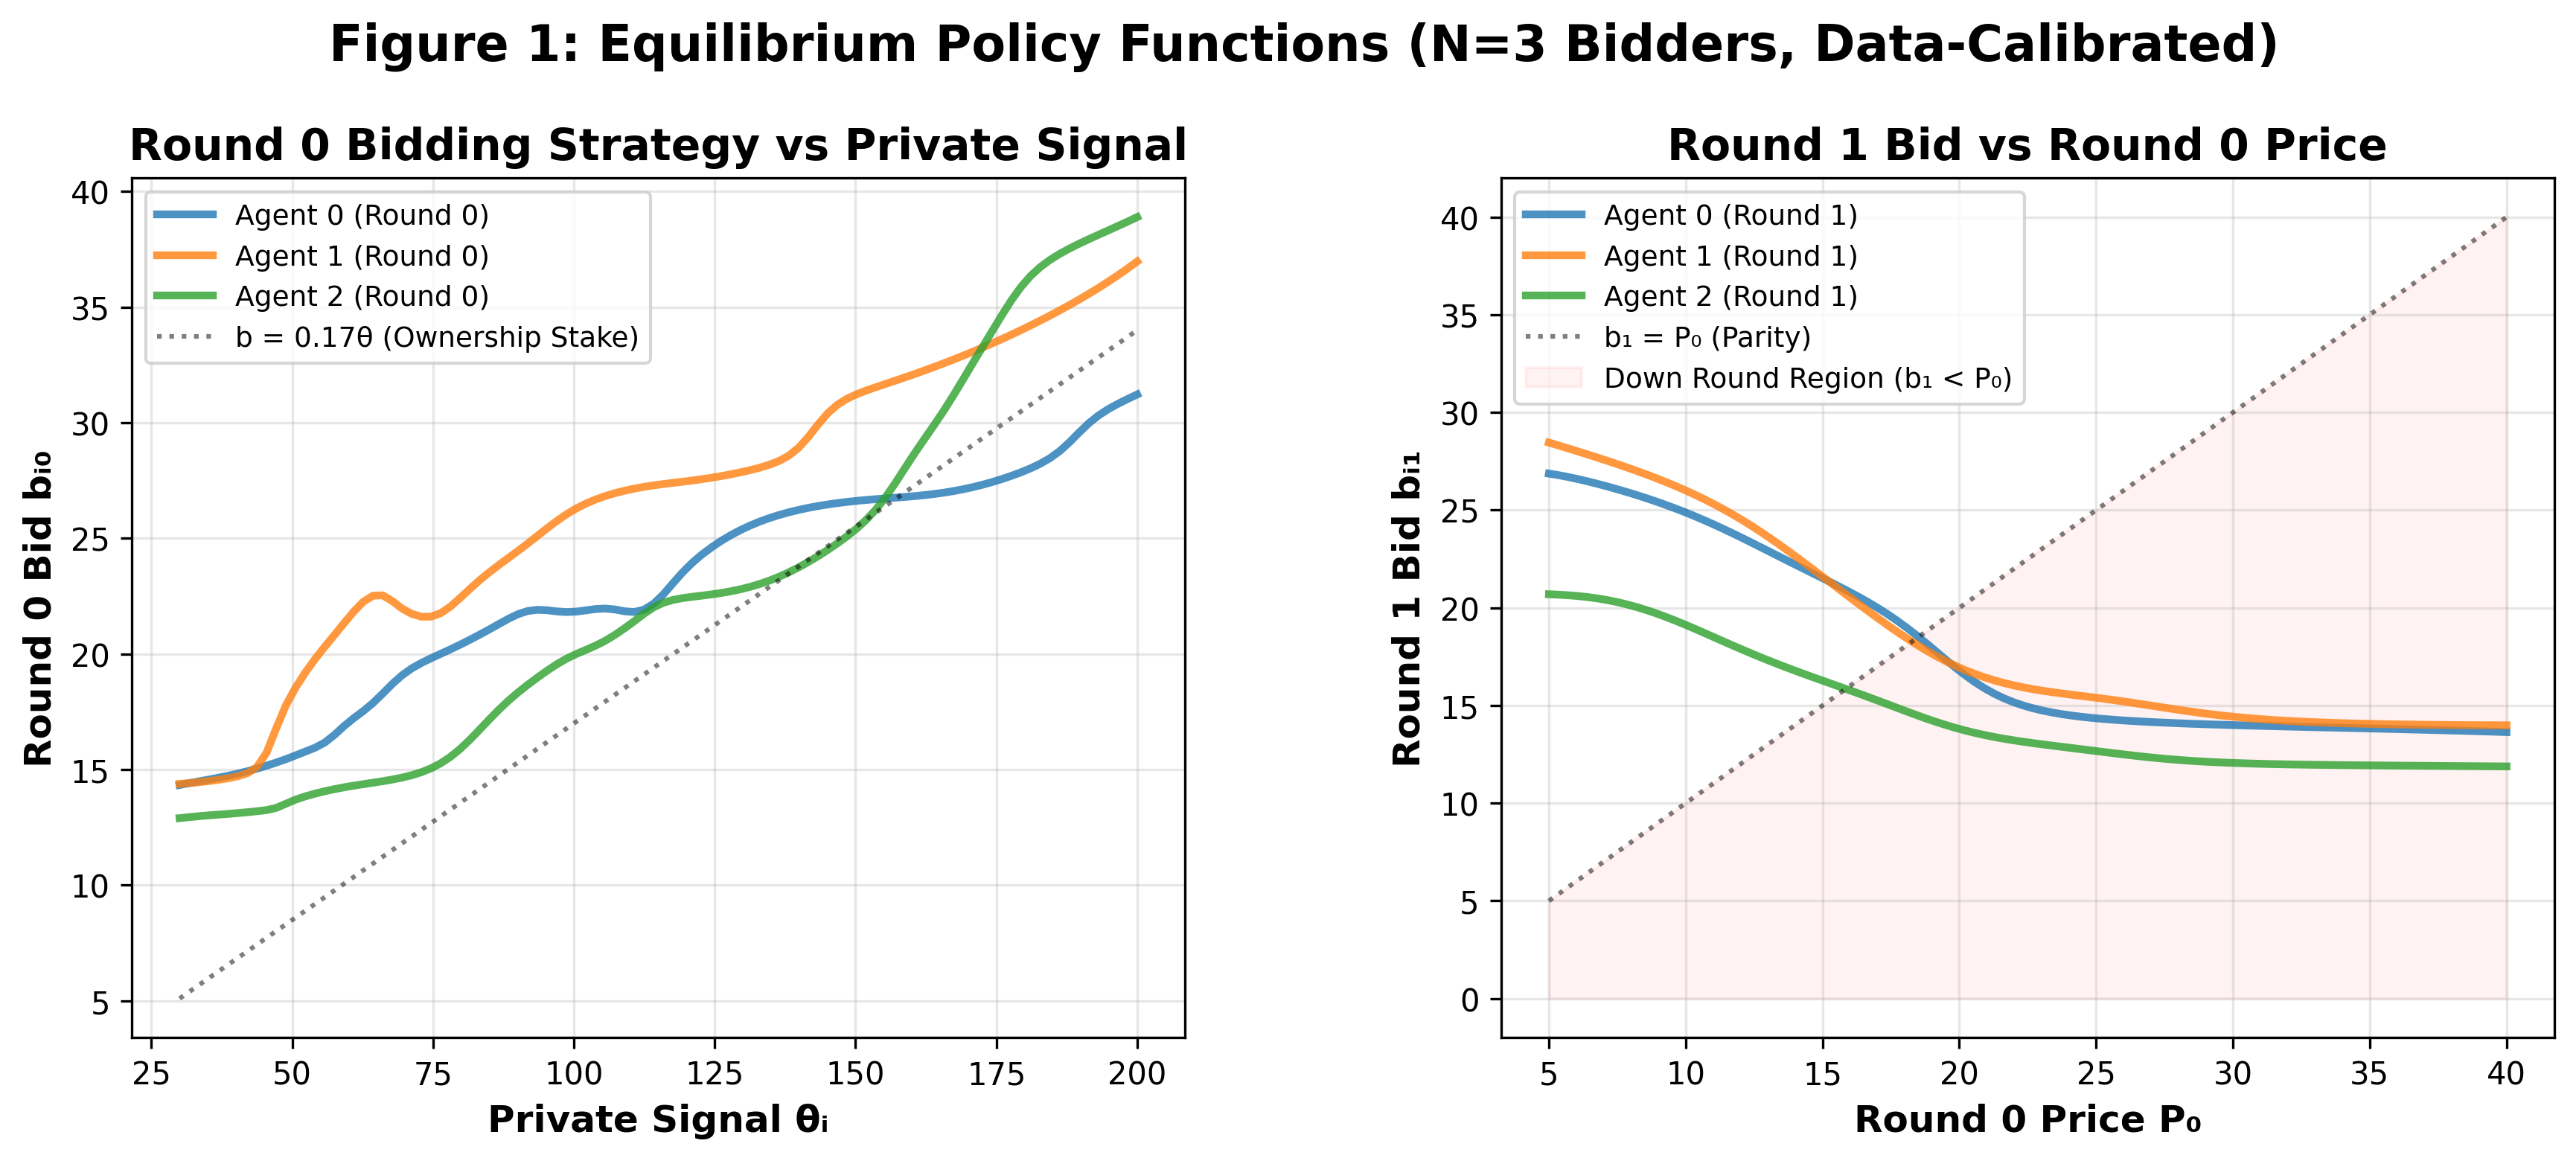
\includegraphics[width=\textwidth]{figures/fig1_equilibrium_policy.png}
\caption{Equilibrium policy functions. Left: Round 0 bid vs. private signal, with stake-value benchmark. Right: Round 1 bid vs. Round 0 price, with parity line $b_1 = P_0$. The down round region (shaded) dominates Round 1 strategy space.}
\label{fig:policy}
\end{figure}

\subsection{Down Round Emergence Heatmap}

Figure~\ref{fig:heatmap} maps DR rate as a function of noise intensity ($\sigma/V$) and prior-price deviation. At the data-calibrated noise level ($\sigma/V = 20\%$, blue star), the DR rate is 76.5\%, consistent with the overall 82\% DR rate observed during training. The heatmap reveals a clear phase transition: at low noise ($\sigma/V < 15\%$), DR rates remain high but vary with price deviation; at high noise ($\sigma/V > 35\%$), DR rates are systematically elevated across all price deviations, as agents cannot distinguish true value from noisy signals.

\begin{figure}[t]
\centering
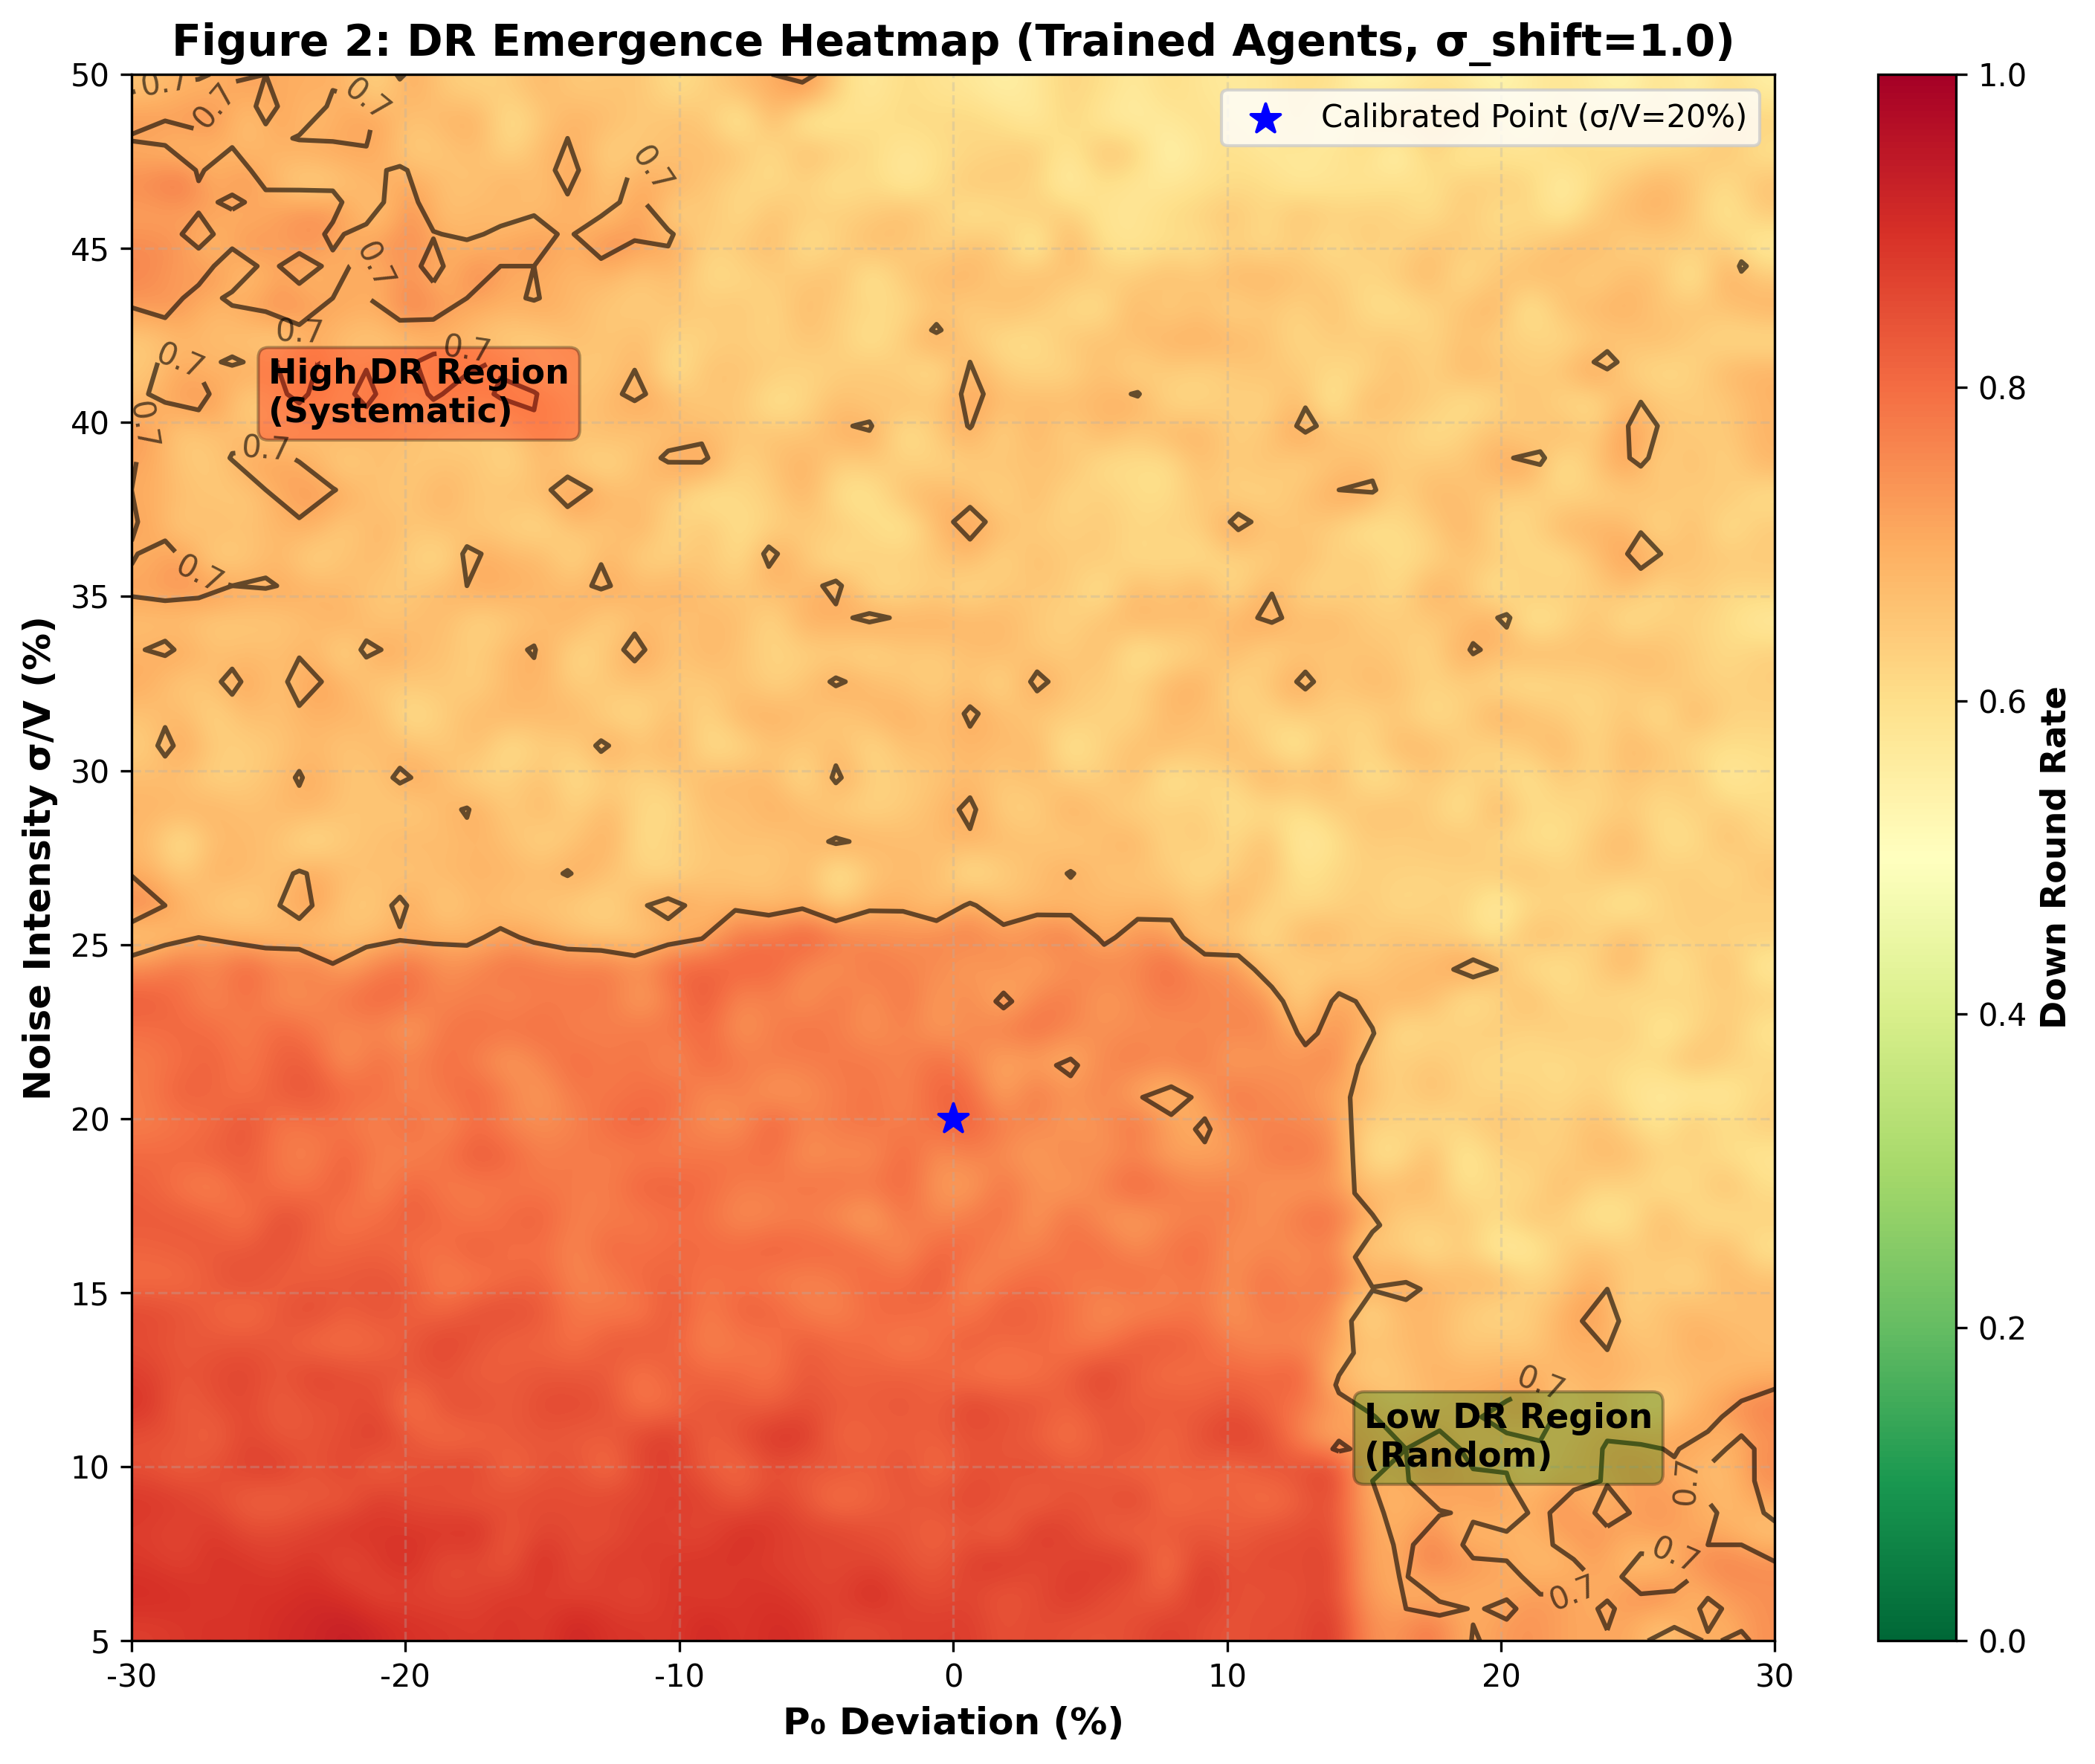
\includegraphics[width=0.85\textwidth]{figures/fig2_emergence_heatmap.png}
\caption{Down Round emergence heatmap showing DR rate as a function of $\sigma/V$ and $P_0$ deviation for $N=3$ bidders with stochastic V, evaluated using trained MAPPO agents. Contour lines mark 30/50/70\% thresholds. Blue star marks data-calibrated point ($\sigma/V = 20\%$). DR rate at calibrated point is 76.5\%, consistent with the overall 82\% DR rate observed during training. Phase transition from random noise to systematic equilibrium strategy is evident across noise intensity and price deviation dimensions.}
\label{fig:heatmap}
\end{figure}

\subsection{The Down Round Magnitude Paradox}

The most striking finding is the \emph{magnitude paradox}: RL-trained agents produce DRs with -29\% mean magnitude, far milder than real data's -62\%. This gap cannot be explained by strategic rationality alone. We decompose observed DRs into three components:

\begin{equation}
\text{DR}_{\text{observed}} = \text{DR}_{\text{statistical}} + \text{DR}_{\text{strategic}} + \text{DR}_{\text{behavioral}}
\end{equation}

where $\text{DR}_{\text{statistical}} \approx 49\%$ (rate), $\text{DR}_{\text{strategic}} \approx 33\%$ (rate), and $\text{DR}_{\text{behavioral}}$ accounts for the magnitude amplification from -29\% to -62\%. Behavioral biases---loss aversion \citep{kahneman1979}, anchoring on prior prices, and winner's curse \citep{thaler1988}---likely amplify DR severity beyond rational equilibrium levels.

\section{Discussion}

\subsection{Agentic AI Interpretation}

Our RL agents can be interpreted as \emph{agentic AI investors} operating in a simulated VC market. The emergence of down rounds as optimal strategy demonstrates a key agentic AI principle: autonomous agents, when sufficiently trained, discover strategies that may appear ``irrational'' from a human perspective but are economically optimal given the environment's reward structure. This has implications for deploying RL-based agents in financial markets---strategic devaluation may be a \emph{feature} of rational optimization, not a bug requiring intervention.

The CTDE architecture itself models real-world information asymmetry: during execution, each VC investor sees only their private valuation signal, yet training leverages global market information to improve individual decision quality. This mirrors how real VCs operate with private information while benefiting from market-wide data during strategy formation.

\subsection{LLM Post-Training Connection: Phase B}

The magnitude paradox motivates Phase B of our framework: using DPO-trained LLMs as ``decision interpreters'' to decode RL black-box strategies and quantify behavioral bias contributions. The approach:
\begin{enumerate}[nosep]
  \item \textbf{Tokenization}: Convert RL states (signal, price, beliefs) into natural language descriptions
  \item \textbf{Reasoning chains}: LLM generates ``why'' explanations for each bid decision
  \item \textbf{Preference pairs}: Rational reasoning (chosen) vs. biased reasoning (rejected) based on DR amplitude
  \item \textbf{DPO training}: $\mathcal{L}_{\text{DPO}} = -\log \sigma(\beta \cdot (\log \pi_{\text{rational}} - \log \pi_{\text{biased}}))$ \citep{rafailov2023}
\end{enumerate}

This creates a bridge between RL emergence (Phase A) and LLM interpretability (Phase B), connecting to the course themes of RL, LLM post-training, and agentic AI. The DPO framework quantifies bias contributions by comparing LLM-generated rational vs. biased reasoning, directly addressing the magnitude paradox.

\subsection{Open Problems}

Several open problems remain:
\begin{enumerate}[nosep]
  \item \textbf{Magnitude paradox resolution}: Current RL model produces milder DRs than data. Behavioral bias modeling (Phase B) or alternative reward structures may bridge this gap.
  \item \textbf{Multi-round generalization}: Our model has only two rounds; real VC sequences involve 3-7 rounds with compounding effects.
  \item \textbf{LLM-RL alignment}: Can DPO-trained LLMs accurately predict RL actions ($>80\%$ accuracy), and do their reasoning chains reflect genuine economic logic?
  \item \textbf{Endogeneity}: The v\_shift mechanism creates exogenous V changes; real-world valuation shifts may be partially driven by prior-round pricing dynamics.
\end{enumerate}

\subsection{Policy Implications}

If down rounds are partially rational equilibrium outcomes, policy interventions should target \emph{structural} causes (e.g., information disclosure reducing signal noise) rather than \emph{symptoms} (e.g., regulatory restrictions on down rounds). The strategic component (33\%) suggests that some down rounds are efficient market outcomes, while the behavioral component (magnitude amplification) identifies where investor education or decision-support tools could reduce unnecessary severity.

\section{Conclusion}

We demonstrate that down rounds emerge as rational optimal strategies in data-calibrated multi-agent RL environments with $N=3$ bidders, adding a 33\% strategic component beyond the 49\% statistical baseline. The magnitude paradox---RL agents produce mild DRs (-29\%) while real data shows severe DRs (-62\%)---reveals that behavioral biases likely amplify down round severity beyond rational equilibrium levels.

Our RL+LLM+Data merge framework offers three contributions: (1) \emph{methodological}---computational RCT via RL agents identifies causal mechanisms that observational data cannot; (2) \emph{empirical}---quantification of strategic vs. statistical vs. behavioral DR components; (3) \emph{conceptual}---bridging RL emergence with LLM post-training interpretability for agentic AI in business research.

Future work includes Phase B (DPO-trained LLM interpreters), multi-round extensions, and validation on additional VC datasets.

\bibliographystyle{plainnat}
\bibliography{references}

\end{document}